%%%%%%%%%%%%%%%%%%%%%%%%%%%%%%%%%%%%%%%%%%%%%%%%%%%%%%%
%%%  Exploring the Semantic Context of News Events  %%%
%%%%%%%%%%%%%%%%%%%%%%%%%%%%%%%%%%%%%%%%%%%%%%%%%%%%%%%

\documentclass{llncs}

\newcommand{\superscript}[1]{\ensuremath{^{\textrm{#1}}}}

\usepackage{makeidx}  % allows for indexgeneration
\usepackage[hyphens]{url}
\usepackage{textcomp}
\usepackage{color}
\usepackage{listings}
\usepackage{multirow}
\usepackage{mathtools}
\usepackage{graphicx}
\usepackage{fancyvrb}
\usepackage{amsmath}
\usepackage{graphicx}
\usepackage[font=small,labelfont=bf]{caption}
\usepackage{pbox}
\usepackage{amsfonts}
\newcommand{\hg}[1]{\colorbox{yellow}{#1}}
\newcommand{\todo}[1]{\colorbox{red}{#1}}

\setcounter{MaxMatrixCols}{20}

% listing styles
\lstset{numbers=left, numberstyle=\tiny,basicstyle=\ttfamily\scriptsize, tabsize=2, keywordstyle=\underbar, stringstyle=\small, backgroundcolor=\color[gray]{0.94}, framexleftmargin=2pt}
\lstdefinestyle{rdfa}{numberblanklines=true, morekeywords={}}

%%%%%%%%%%%%%%%%%%%%%%%%
%%%  Begin Document  %%%
%%%%%%%%%%%%%%%%%%%%%%%%

\begin{document}

\frontmatter          % for the preliminaries
\pagestyle{headings}  % switches on printing of running heads
\mainmatter              % start of the contributions

%\title{Exploring the Semantic Context of News Events}
%\title{Spotting the Hidden Semantics of Newscasts}
\title{Generating Semantic Snapshots of Newscasts using Entity Expansion}
\author{Jos\'e Luis Redondo Garc\'ia\inst{1}, Giuseppe Rizzo\inst{1}, Lilia Perez Romero\inst{2}, Michiel Hildebrand\inst{2}, Rapha\"el Troncy\inst{1}}
\institute{EURECOM, Sophia Antipolis, France, \\
\email{\{redondo, giuseppe.rizzo, raphael.troncy\}@eurecom.fr}
\and
CWI, Amsterdam, The Netherlands, \\
\email{\{L.Perez, M.Hildebrand\}@cwi.nl}
}

\maketitle              % typeset the title of the contribution

%%%%%%%%%%%%%%%%%%
%%%  Abstract  %%%
%%%%%%%%%%%%%%%%%%

\begin{abstract}

% A recent trend in the newscasts domain consists on developing second screen applications that enable the user to further dive and improve his understanding of some particular news items, specially the complex word-scale controversial ones. The making of such applications requires the semantic annotation of the original newscasts as well as semantic enrichment for including background knowledge. Relying on video subtitles for providing time-based annotations of video content is a common method. However, it is insufficient to fully grasp the context of the newscasts being reported, simply because daily news reporting emphasizes on the last facts rather than on the narrative and causes of the reported event. In this paper, we propose a method that enables to search for and analyze related documents in order to generate semantic annotations that are closer to what viewers and experts in the domain expect to find while consuming newscasts. This approach generates annotations in the form of a ranked list of entities. We evaluate this method with respect to a gold standard made by domain experts for a set of BBC newscasts. Results of the experiments show the robustness in semantically annotating newscasts holding an Average Normalized Discounted Cumulative Gain of 66.4\%.

Television newscasts generally report about the latest event-related facts occurring in the world. \textit{Per se} a newscast delivers partial information thus neglecting the whole picture of the event that is often assumed as known. Relying exclusively on the broadcasted news item is therefore insufficient to fully grasp the context of the fact being reported. In this paper, we propose an approach to retrieve and analyze related documents in order to automatically generate semantic annotations that provide viewers and experts of the domain comprehensive information to fully understand the news content. The approach takes as inputs the publication date and the newscast's title for gathering event-related documents on the Web, bringing more representativeness to the available knowledge. Then named entities detected in the retrieved documents are merged with those found in the newscast subtitles for further disclosing hidden relevant entities that were not explicitly mentioned in the original newscast. A ranking algorithm based on entity frequency, popularity peak analysis, and domain experts' rules sorts the annotations to generate the Semantic Snapshot of the considered Newscast (NSS). We benchmark this method against a gold standard generated by domain experts and assessed via a user survey over five BBC newscasts. Results of the experiments show the robustness of the approach holding an Average Normalized Discounted Cumulative Gain of 66.6\%.
%Lilia: not sure whether we can call our videos newscasts or whether they are more online news videos
\keywords{Semantic Video Annotation, Entity Expansion, Newscasts}
\end{abstract}

%%%%%%%%%%%%%%%%%%%%%%%%%
%%%  1. Introduction  %%%
%%%%%%%%%%%%%%%%%%%%%%%%%
\section{Introduction}
\label{sec:introduction}
With the emergence of both citizen-based and social media, traditional information television channels have to re-think their production and distribution workflow processes. We live in a globalized world, a vast playing field where events happening are the result of complex interactions between many diverse agents along time. The interpretation of those news is problematic because of two issues. \textit{i)} the \textit{need of background}: viewers probably need to be aware of other facts happened in a different temporal or geographic dimension.
%, like one week ago or in a completely different region. 
\textit{ii)} the \textit{need of completeness}: a single representation of an event is not enough to capture the whole picture, because it is normally incomplete, it can be biased, or partially wrong. 
Recent gadgets and applications, such as second screen devices, have recently irrupt as a good way of assisting the viewer in the challenge of becoming aware of
that bigger picture of the event. In~\cite{Courtois2012}, the authors tracked 260 tablet users, concluding that even though there is a modest uptake and interest in using secondary screens to digitally share opinions, the use of second screen interaction with television content is something the viewer qualitatively appreciate.
%In addition, traditional text-based products are losing market share against other audiovisual solutions, in particular video. 
But there is still a crucial aspect open: the second screen interaction needs to be fed with meaningful details concerning a newscast. The most common strategy to get this information is to enrich the original content with additional data collected from external sources. Today users have access to multiple news portals, different services for commenting and debating on the news, and social media that instantaneously spread news information. However, this results in large amounts of unreliable and repeated information, leaving to the user the burden of processing the large amounts of potentially related data to build an understanding of the event.
%in the middle of an ocean of rumors or hoaxes.

%\todo{GR: this is a jump -> from means (video, ...) to entities so why?}
Machine driven approaches have tried to alleviate the human difficulties when navigating this huge amount of data, but they struggle both in finding a good set of candidate documents, and filtering them.
% in order to offer relevant data back to the users. 
One strategy reported in the literature for having such a mechanism is to perform named entity extraction over the newscast transcript~\cite{Yunjia2012}. However, the set of named entities obtained from such an operation is insufficient and incomplete for expressing the context of a news event~\cite{Henzinger2003}. Sometimes entities spotted over a particular document are not disambiguated because the textual clues surrounding the entity are not precise enough for the name entity extractor. While in some others, entities are simply not mentioned in the transcripts while being relevant for understanding the story. This is also an inherent problem in information retrieval tasks: a single description about the same resource does not necessarily summarize the whole picture. In this paper we automatically retrieve and analyze additional documents from the Web where the same event is also described, in a process called Newscast Named Entity Expansion. By increasing the size of the document set to analyze, we increase the completeness of the context and the representativeness of the list of entities, reinforcing relevant entities and finding new ones that are potentially interesting inside the context of that news item. This approach is able to produce a ranked list of entities called Newscast Semantic Snapshot (NSS), which includes the initial set of detected entities in subtitles with other event-related entities captured from the seed documents. 
%The NSS is later used to feed second screen applications assisting the consumer who watches the news, summarizing and generating quality snippets, or launch further  enrichment processes who bring related content the users could be also interested in watch. 

The paper is organized as follows: Section~\ref{sec:RelatedWork} presents the related works, Section~\ref{sec:Approach} illustrates the approach depicted in this paper for generating NSS. Section~\ref{sec:Ranking} describes in depth the different ranking algorithms used for ordering the list of candidate entities generated in previous steps. In Section~\ref{sec:GoldStandard} we report about the creation of the gold standard used for evaluating the NSS. The experimental settings are described in Section~\ref{sec:Evaluation}. We conclude with Section~\ref{sec:Conclusion} summarizing the main findings and outlining the future plans.

% State of the Art on Semantic annotation
%* State of the Art on Semantic annotation.
%Concerning the multimedia annotation the literature covers a wide range of different analysis techniques~\cite{ballan2011event}. One of the main approaches consists on running Named Entity Recognition (NER) over the textual information attached to particular video fragment. Those techniques are an essential component within the Information Extraction field that focus on: identifying atomic information units in texts, named entities; classifying entities into predefined categories (also called context types) and linking to real world objects using web identifiers (Named Entity Disambiguation). A growing number of APIs provide such a service, like AlchemyAPI\footnote{\fontsize{8pt}{1em}\selectfont \url{http://www.alchemyapi.com/}} or DBpedia Spotlight\footnote{\fontsize{8pt}{1em}\selectfont \url{http://spotlight.dbpedia.org/}}. 


%%%%%%%%%%%%%%%%%%%%%%%%%
%%%  2. Related Work  %%%
%%%%%%%%%%%%%%%%%%%%%%%%%

\section{Related Work}
\label{sec:RelatedWork}
%Studies on second screen applications and tools for supporting journalists. (WHY)
%\todo{GR:the first 4 lines are simply blabla and can be removed without loss}
%Television content in general and newscast in particular need the assistance of innovative applications which help the viewers and experts to get the most of them. One implementation design that has been deeply studied in the last years, mainly due to the increasing availability of tablets and tactile device is the "second screen application" paradigm. This kind of experiences open new possibilities for users watching television by complementing what is being displayed on the screen and offering a more active interaction with the content. 

%The need of a semantic snapshot.
The need of a NSS for feeding certain applications is already a concept we have investigated in previous research works and prototypes \cite{Redondo2014}, which have probed the benefit for users of browsing the ``surrounding context'' of the newscasts. The same concept\footnote{\url{https://vimeo.com/119107849}} has been presented to the forum Iberoamerican Biennial of Design (BID).\footnote{\url{http://www.bid-dimad.org}} with great feedback from users and experts.
% with great reviews from the experts and scoring between the final 5 from a total of 200 candidates. \\
Research efforts have underlined the importance in professional journalism of algorithms, data, and social science methods for reporting and storytelling, under the term of computational exploration in journalism ~\cite{gynnild2014}.  %CEJ demands precise event descriptions for supporting the journalistic co-creation of quantitative news projects that transcend geographical, disciplinary, and linguistic boundaries.
%%Entities in making sense (Semantic snapshot)  (WHAT)
%All those news applications need to be fed with the appropriate data to effectively assist viewers and professionals, and this information is normally broader than the one explicitly offered by the content itself. The hypothesis presented in this research paper states that this required knowledge can be represented in the form of a list of named entities called Newscast Semantic Snapshot (NSS). 
%This idea of using semantic annotations and named entities in particular is not new. 
Projects like NEWs have studied how to disambiguate named entity in the news domain by continuously learning while processing news streams~\cite{Fernandez2012}. In the domain of Social Networks, named entities are also used for identifying and modeling events and detecting breaking news. In~\cite{Steiner2013}, the authors emphasize the importance of spotting news entities in short user generated post in order to obtain a better understanding about what they are talking about. Entities have been used for the video classification when the textual information attached to a video contains temporal references (e.g. subtitles)~\cite{yunjia2013}. 

%How to create this semantic snapshot (Expansion idea) (HOW)
In order to build a comprehensive NSS the knowledge expressed in the newscast has to be extended with further entities that are not explicitly mentioned in the video item. Our approach performs an entity expansion process, which allows to collect on the fly event-related documents from the Web. In the literature there are already some approaches relying in similar expansion techniques, even if the final objective is not spotting other event-related entities: instead, they transform the feature space from a from small number of named entities with the same type or category to a more complete named entity set. One of them is Google Sets.\footnote{\url{http://googlesystem.blogspot.fr/2012/11/google-sets-still-available.html} not longer available since 2014.} Set expansion using the Web is also closely related to the problem of unsupervised relation learning~\cite{Cafarella2005}, and set-expansion-like techniques have been used to derive features for concept-learning~\cite{Cohen2000}, to construct ``pseudo-users'' for collaborative filtering~\cite{Cohen99}, and to compute similarity between attribute values in autonomous databases~\cite{Wolf2007}. In~\cite{Wang2007}, authors proposed the Set Expander for Any Language (SEAL) approach. SEAL works by automatically finding semi-structured web pages that contain lists of items and the aggregating these list in a way that the most promising items are ranked higher. SEAL is a language-independent system and it has shown good performance against previously published results like the already mentioned Google Sets. By using particular seeds and the top one hundred documents returned by Google, SEAL achieves 93\% in average precision in dataset from various languages. The same authors published an improved version of the algorithm~\cite{Wang2008}, increasing the performance by handling unlimited number of supervised seeds. In each iteration, it expands a couple of randomly selected seeds while accumulating statistics from one iteration to another. Our approach does not rely on such kind of iterative mechanism, and focus more in maximize the quality of the search query for obtaining the most appropriate set of related documents to be analyzed. Another approach in extending set of entities is \cite{Mai-Vu2010}, which combines the power of semantic relations between language terms like synonymy and hyponymy and grammar rules in order to find additional entities in the Web sharing the same category that the ones provides as input. Relying in Google they analyze documents for parsing semistructured text elements like tables and rank the final candidates using different ranking algorithms like PageRank. Numerous approaches have dealt with a set expansion method using free text rather than semi-structured Web documents; for instance authors in \cite{Talukdar2006} presented a method for automatically selecting trigger words to mark the beginning of a pattern, which is then used for bootstrapping from free text. But still this approach looks for category related entities while in our case the driving force is more the event being shown in the news item. To the best of our knowledge, the only related work in the news domain that has been carried out grounding the power of enriching the set of initial entities by using an entity expansion algorithm is~\cite{RedondoGarcia2014}. It includes a naive document collection strategy, it proposes an entity ranking algorithm based on the appearance of the entities in the collected documents, and it exploits the DBpedia knowledge base as a way to ensure the coherence of the final list of entities. The work presented in this paper improves the referred work in several directions: document retrieval mechanism, semantic annotation, creation of the NSS. \cite{RedondoGarcia2014} is used as one of the baselines in the experimental settings.%\hg{they are missing some examples of SSN and the related work made by Lilia}.

%%%%%%%%%%%%%%%%%%%%%%%%%%%%%%%%%%%%%%%%%%%%
%%%  3. News Concept Expansion Approach  %%%
%%%%%%%%%%%%%%%%%%%%%%%%%%%%%%%%%%%%%%%%%%%%
\section{Newscast Entity Expansion Approach}
\label{sec:Approach}
%In this section we present our algorithm to automatically generate News Semantic Snapshots out of a particular newscast. 
The approach we use to generate Newscast Semantic Snapshot is composed of the following stages: query formulation, document retrieval, semantic annotation, annotation filtering, and annotation ranking. Fig.~\ref{fig:namedEntityExpansion} depicts the whole expansion process.
\begin{figure}[h!]
\centering
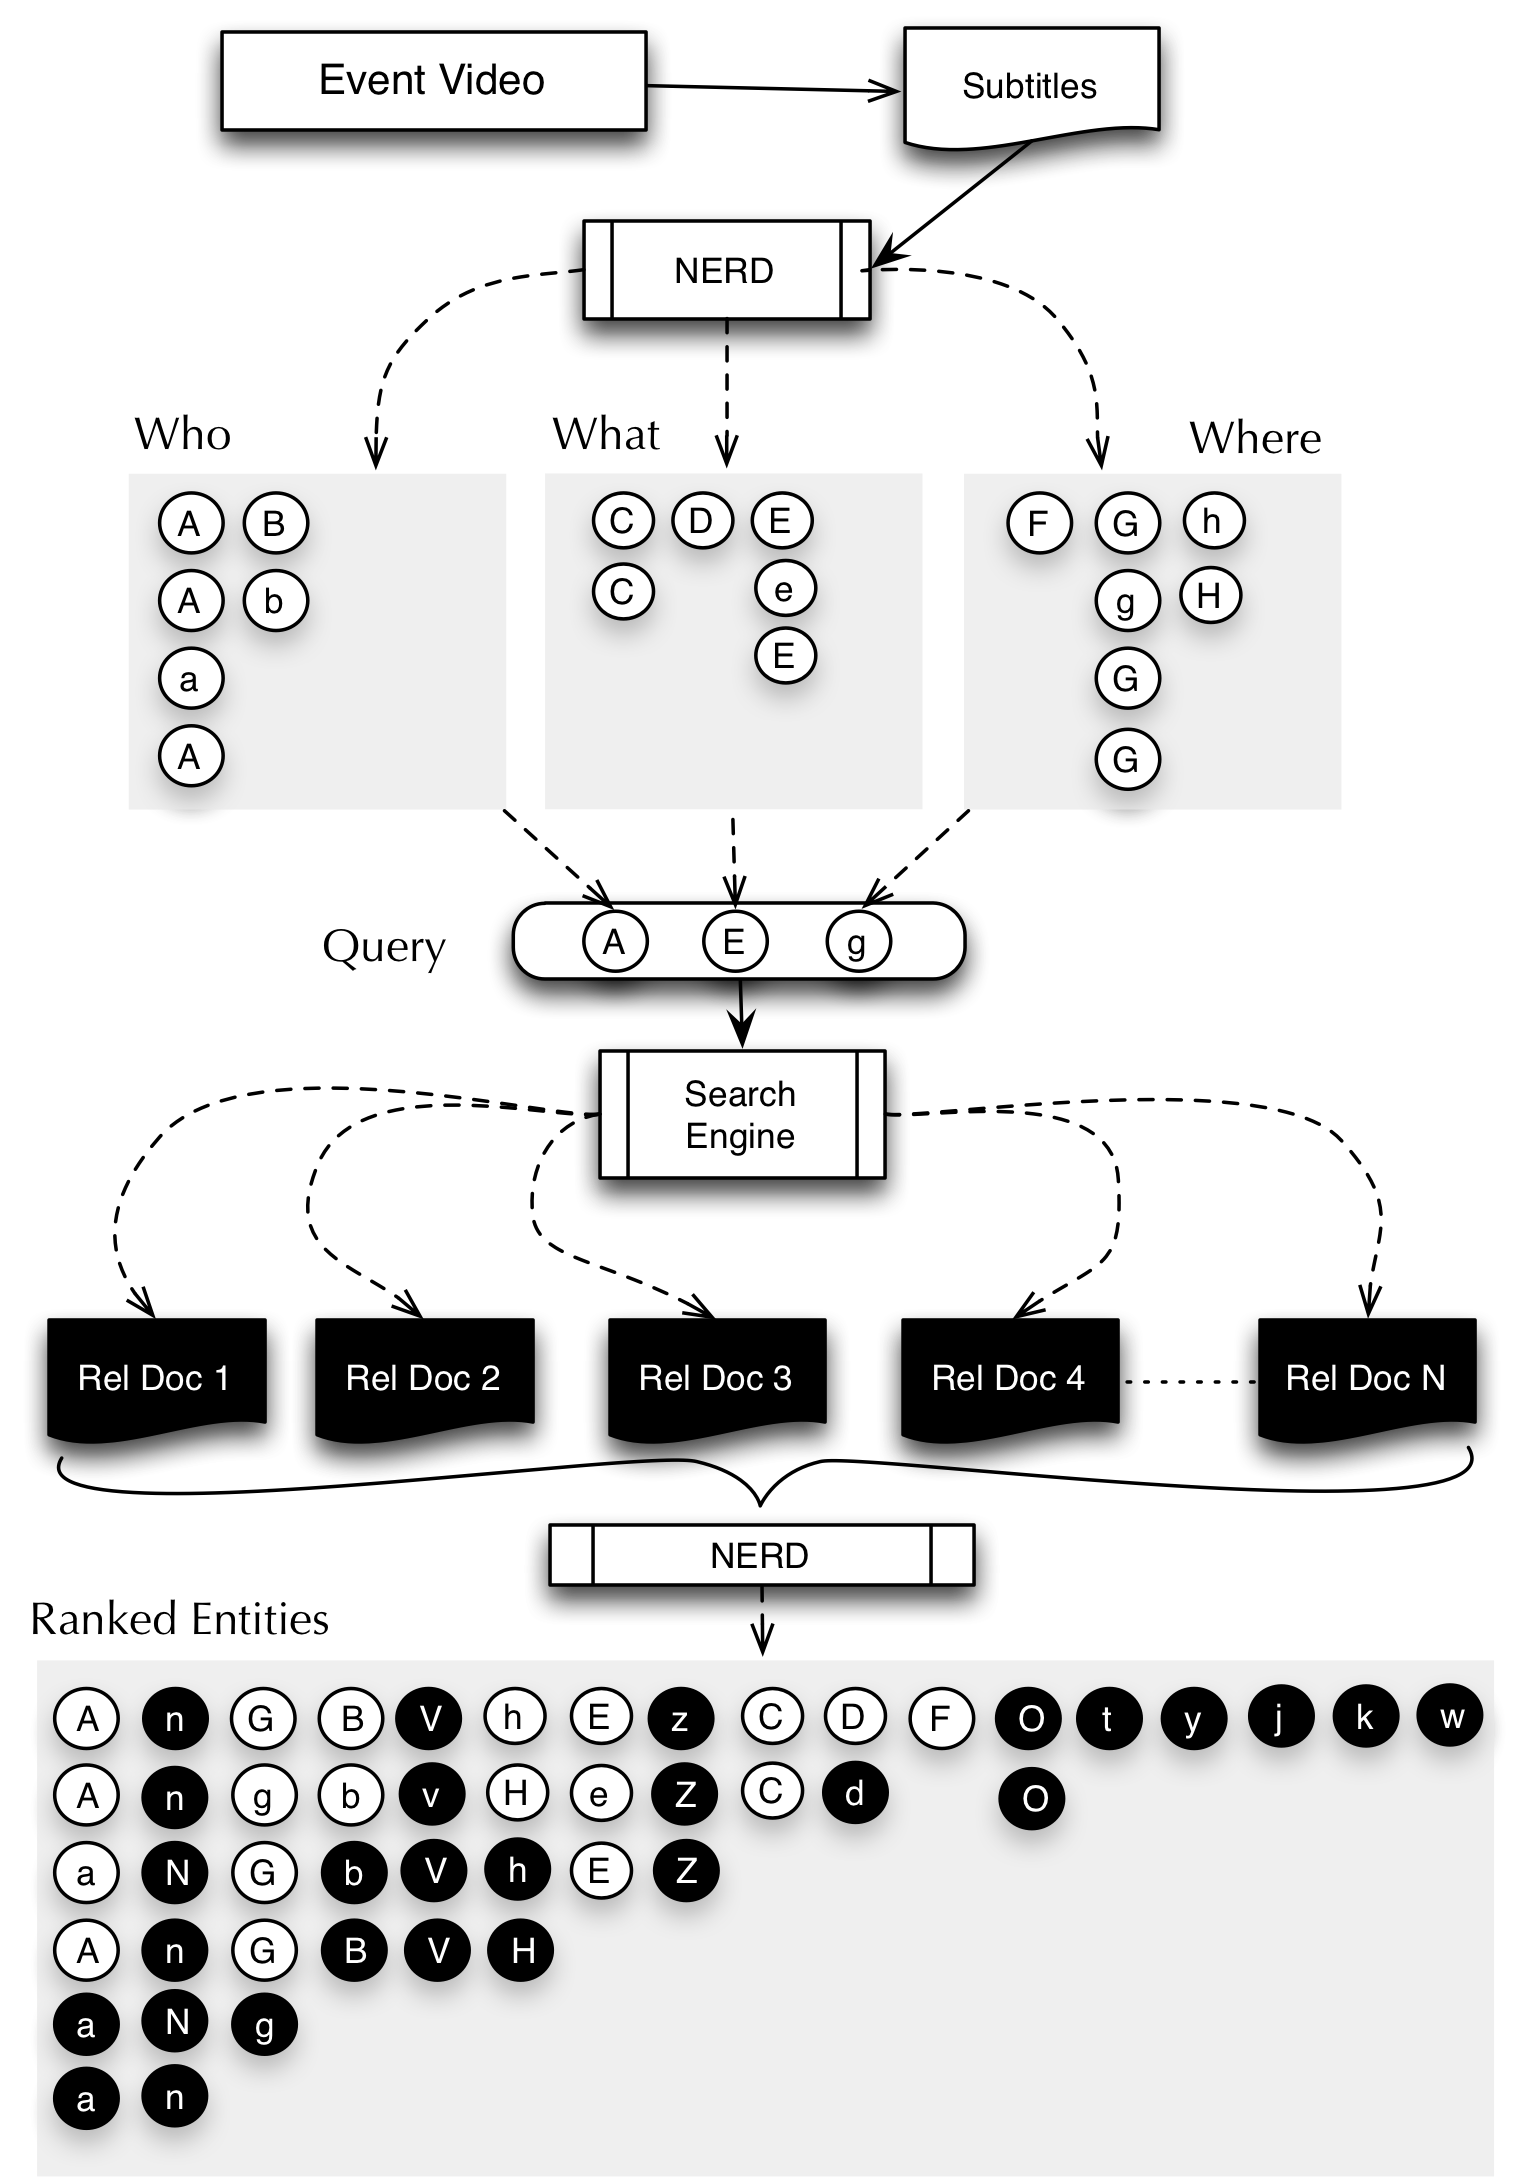
\includegraphics[width=1\textwidth]{figure/ExpansionDiagram}
\caption{Schema of Named Entity Expansion Algorithm.}
\label{fig:namedEntityExpansion}%\end{figure}
\end{figure}

{\bf Query Formulation} %OLD APPROACH
%The \emph{Five W's} is a popular concept of information gathering in journalistic reporting. It captures the main aspects of a story: who, when, what, where, and why~\cite{LiJia2007}. We try to represent the news item in terms of four of those five W's (who is involved in the event, where the event is taking place, what the event is about, and when it has happened) in order to generate a query that retrieves documents associated to the same event.
%First, the original entities are mapped to the NERD Core ontology, which considers 10 main classes: Thing, Amount, Animal, Event, Function, Organization, Location, Person, Product and Time. From those ten different categories, we generalize to three classes: the Who from \url{nerd:Person} and \url{nerd:Organization}, the Where from \url{nerd:Location}, and the What from the rest of NERD types after discarding \url{nerd:Time} and \url{nerd:Amount}.
Newscast broadcasters offer a certain amount of metadata about the items they publish, which is normally available together with the audiovisual content itself. In this work, we build the query $q= \left [ \text{h}, \text{t} \right ]$, where \textit{h} is the video heading, and \textit{t} is the publication date. The query is then used to as input of the retrieval stage.
%newscasts have with the following metadata: title, publication date, and the video transcript (non necessary timed). 
%We model a newscast as:
%\begin{equation}
%\text{q} =\left [ \text{t}, \text{d} \right ]
%\end{equation}
%Those different fields are taken from the video publisher and directly used as input for the rest of the expansion workflow without any pre-processing.

{\bf Document Retrieval}
The retrieval stage has the intent to collect event-related documents from the open Web. To some extents this process emulates what a viewer, who misses some details about the news he is watching, does: going to the Web, make a search, and get the most of the top ranked documents. Our programmatic approach emulates this human driven task by analyzing a much bigger set of related documents in a drastically smaller amount of time. The stage consists of retrieving documents that report on the same event discussed in the original video as result of the query \textit{q}. It has an key role in the upcoming semantic annotation stage, since it selects a set of the documents \textit{D} over which the semantic annotation process is performed. The quality and adequacy of the collected documents sets a theoretical limit on how good the process is done. 
%The more appropriate the collection of related document is, the better the final results will be.
%The different behavior of search engines make some alternatives more suitable than others for certain kinds of events. The way the resulting documents change in the search engines for a particular kind of event is a research question that will not be studied in this paper. 

{\bf Semantic Annotation} In this stage we perform a named entity recognition analysis with the objective of reducing the cardinality of the textual content from the set $D$ of documents $\{d_1, ..., d_n, d_{n+1}\}$ where $d_{i=1,..,n}$ defines the $i_{th}$ retrieved document, while $d_{n+1}$ refers to the original newscast transcript. Since most of the retrieved documents are Web pages, HTML tags and other annotations are removed, keeping only the main textual information. The feature space is then reduced and each document $d_i$ is represented by a bag of entities $E_{d_i}={e_{1_{d_i}}, ..., e_{n_{d_i}}}$, where each entity is defined as a triplet $(surface\_form, type, link)$. We perform a union of the obtained bags of named entities resulting in the bag of entities $E$ of the initial query $q$. 

{\bf Annotation Filtering and Clustering} The Document Retrieval stage expands the content niche of the newscast. At this stage we apply coarse-grained filtering of the annotations $E$ obtained from the previous stage, applying a $f\left ( E_{d_i}\right )\rightarrow  E'_{d_i}$ where $\left |E'_{d_i}  \right | < \left |E_{d_i}  \right |$. The filtering stategy grounds on the findings we obtained in the creation of the gold standard. In fact, when watching a newscast viewers better capture Person-type entities, as well as Organization-type and Location-type entities. The rest of less-specific and wider enclosed entities are more vague to be displayed on a television user interface and potentially less relevant for complementing the seed content. 
Named entities are then clustered applying a centroid-based clustering operation. As cluster centroid we consider the entity with the most frequent disambiguation $link$ that also have the most repeated $surface\_form$. As distance metric for comparing the instances, we applied strict string similarity over the $link$, and in case of mismatch, the Jaro-Winkler string distance~\cite{winkler2006overview} over the $surface\_form$. The output of this phase is a list of clusters containing different instances of the same entity.

{\bf Semantic Annotation Ranking}
%The different related documents collected and annotated in previous steps of the expansion algorithm contain the pieces of the puzzle that will allow to re-construct the big picture of the event. Unfortunately, those pieces come wrapped together with other less important parts which are not closely related with the event in particular and need to be put aside. By ranking the concepts, we make easier to (1) identify important entities from those which are, (2) group them in the top positions in order, (3) easy get rid of those which are not relevant to the considered event. The final NSS will be a subset of the top scored entities after the ranking algorithm.
The bag of named entities $E'_{d_i}$ is further processed to promote the named entities which are highly related to the underlined event. To accomplish such an objective, we propose a ranking strategy based on entity appearance in documents, popularity peak analysis, and domain experts' rules sorts the annotations to generate the Semantic Snapshot of the considered Newscast (NSS).

%%%%%%%%%%%%%%%%%%%%%%%%%%%%
%%%  4. Ranking Strategy %%%
%%%%%%%%%%%%%%%%%%%%%%%%%%%%
\section{Ranking Strategy}
\label{sec:Ranking}
The unordered entity list is ranked to promote the entities that are potentially interesting for the viewer. The strategy we present in this work grounds on the assumption that the entities which appear often in the retrieved documents are important. We propose two different scoring functions for weighting the frequency of the entities. We then consider two orthogonal functions which exploit the entity popularity in the event time window, and the domain experts' rules.
%and get rid of the long queue of less relevant concepts and noise generated by during the collection process. At the same time, this is also the most complicated task to perform: while computers are good in processing much large amounts of information and it would be possible to analyze hundreds of related documents, to decide which of the generated entities would be selected as relevant by a human is much more complicated. 

\subsection{Frequency-based Function}
We first rank the entities according to their absolute frequency within the set of retrieved documents $D$. Let define the absolute frequency of the entity $e_i$ in the collection of documents $D$ as $f_a(e_i, D)$, we define the scoring function $S_F = \frac{ f_a(e_i, D) }{ |E| } $, where $|E|$ is the cardinality of all entities spotted across all documents. 
%Following this criteria, the more mentioned an entity is, the higher is will be scored. The opposite occurs to those barely mentioned all along the corpora, which will drop down in the final list of candidates. Therefore we have implemented a ranking strategy that orders entities according to their absolute frequency all over the collected documents: $S_{F}\left ( e \right ) =  f_{a}(e, D)$. 
%A second version of this simple strategy considers also confidence scores coming form the semantic annotation phase, in order to consider the certainty of the spotting process when detecting the entity $R_{score}\left ( e \right ) =  \sum_{1}^{i}c_{e_{i}}$ . 
In Fig.~\ref{fig:rankingStrategies} (a) we can observe how entities with lower absolute frequency are placed at the beginning of the distribution and discarded in the final ranking; instead those with high $S_F$ are in the right side of the plot, being then considered to be part of the NSS.

\subsection{Gaussian-based Function}
The $S_F$ scoring function privileges the entities which appear often. However from the perspective of a television viewer, this is not always true: while it is true that entities appearing in just a few documents are probably irrelevant and not representative enough to be considered in the final results, entities spread all over the whole set of related documents are not necessary something the viewers would need to know about. In fact, they often represent entities that have been so present in media before that they have become too much obvious to the viewer. This scoring function is therefore approximated by a Gaussian curve.
By characterizing the entities in terms of their Bernoulli appearance rate across all documents $f_{doc}(e_i)$, and applying the Gaussian distribution over those values, we  promote entities distributed around the mean $\mu = \frac{|D|}{2}$ , being $|D|$ is the cardinality of the retrieved documents (Fig.~\ref{fig:rankingStrategies} (b)). In particular the scoring function has been formalized as a simplified version of the normal function: $S_G = 1-\left | \frac{ f_{doc}(e_i) }{|D|} -1 \right |$.
\begin{figure}[h!]
\centering
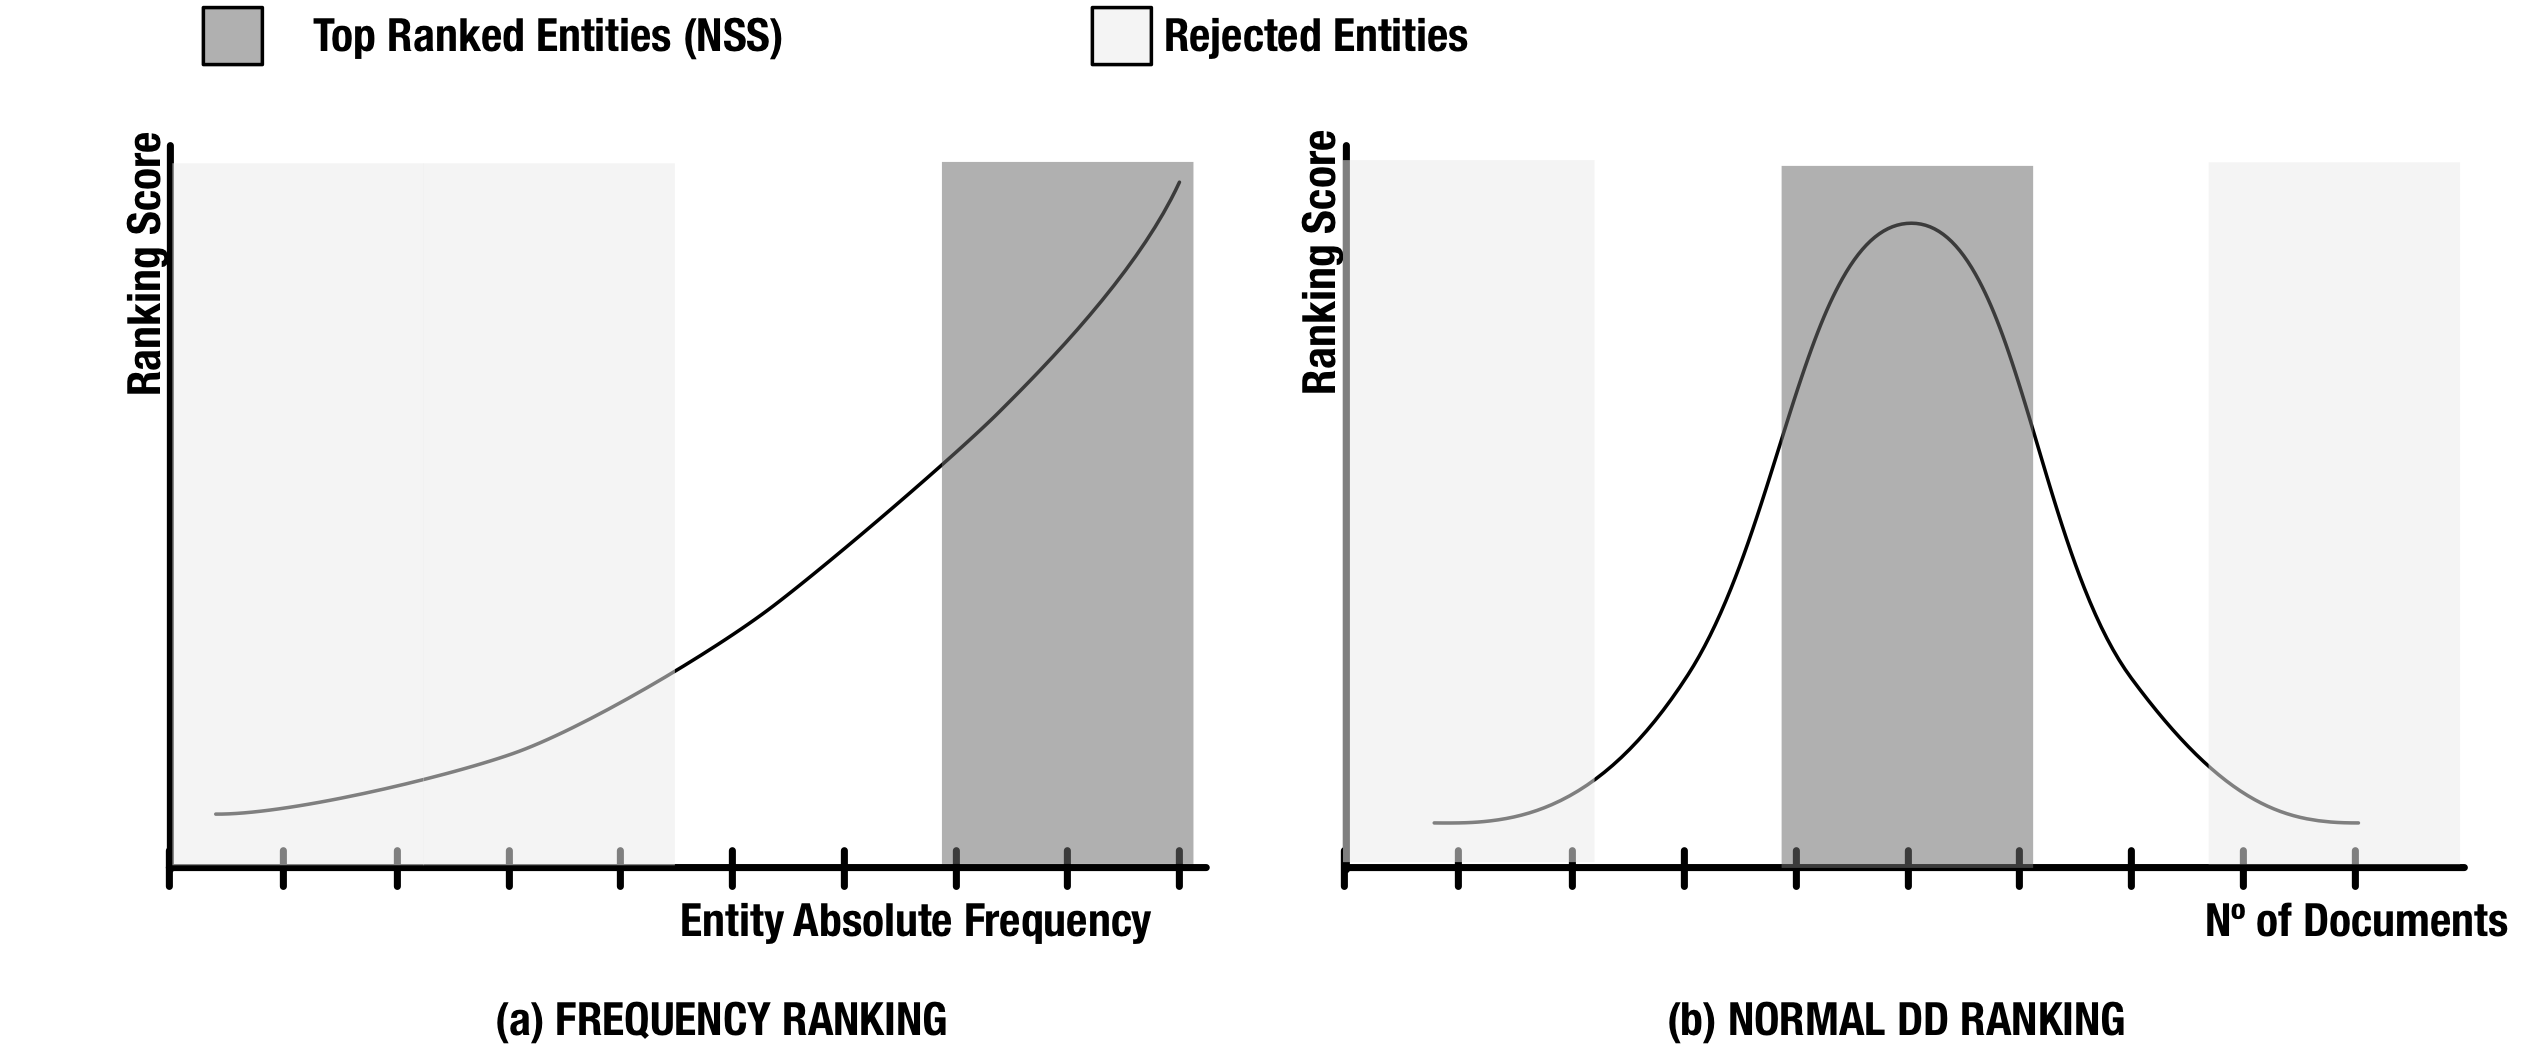
\includegraphics[width=0.9\textwidth]{figure/RankingStrategies}
\caption{(a) depicts the Decay function of the entity occurrences in the corpus, and the $S_F$ which underlines the importance of an entity being used several times in the corpus. (b) represents the Gaussian-based function $S_G$, with the entities highly impontant over the mean.}
\label{fig:rankingStrategies}%\end{figure}
\end{figure}

% Random Walks
% PageRank
% Use prior knowledge graph


\subsection{Orthogonal Functions}
\subsubsection{Popularity Function}
%Even the three ranking algorithms follow different considerations and principles, they end up exploiting the most precise an representative frequency values that the entity expansion process can provide compared to any other analysis over more reduced and probably partial newscast descriptions. 
We propose a weighting function based on a mechanism that detects variations in entity popularity values over a time window (commonly named as popularity peaks) around the date of the studied event. The functions proposed above exploit the frequency of the entities in documents as a factor to measure its importance. However the frequency based approaches fail to explain the phenomenon of certain found entities which are barely mentioned in related documents but suddenly become interesting for viewers. These changes are sometimes unpredictable so the only solution is to rely on external sources that can provide indications about the entity popularity, like Google Trends\footnote{\url{https://www.google.com/trends}} or Twitter.\footnote{\url{https://twitter.com}}
\begin{figure}[h!]
\centering
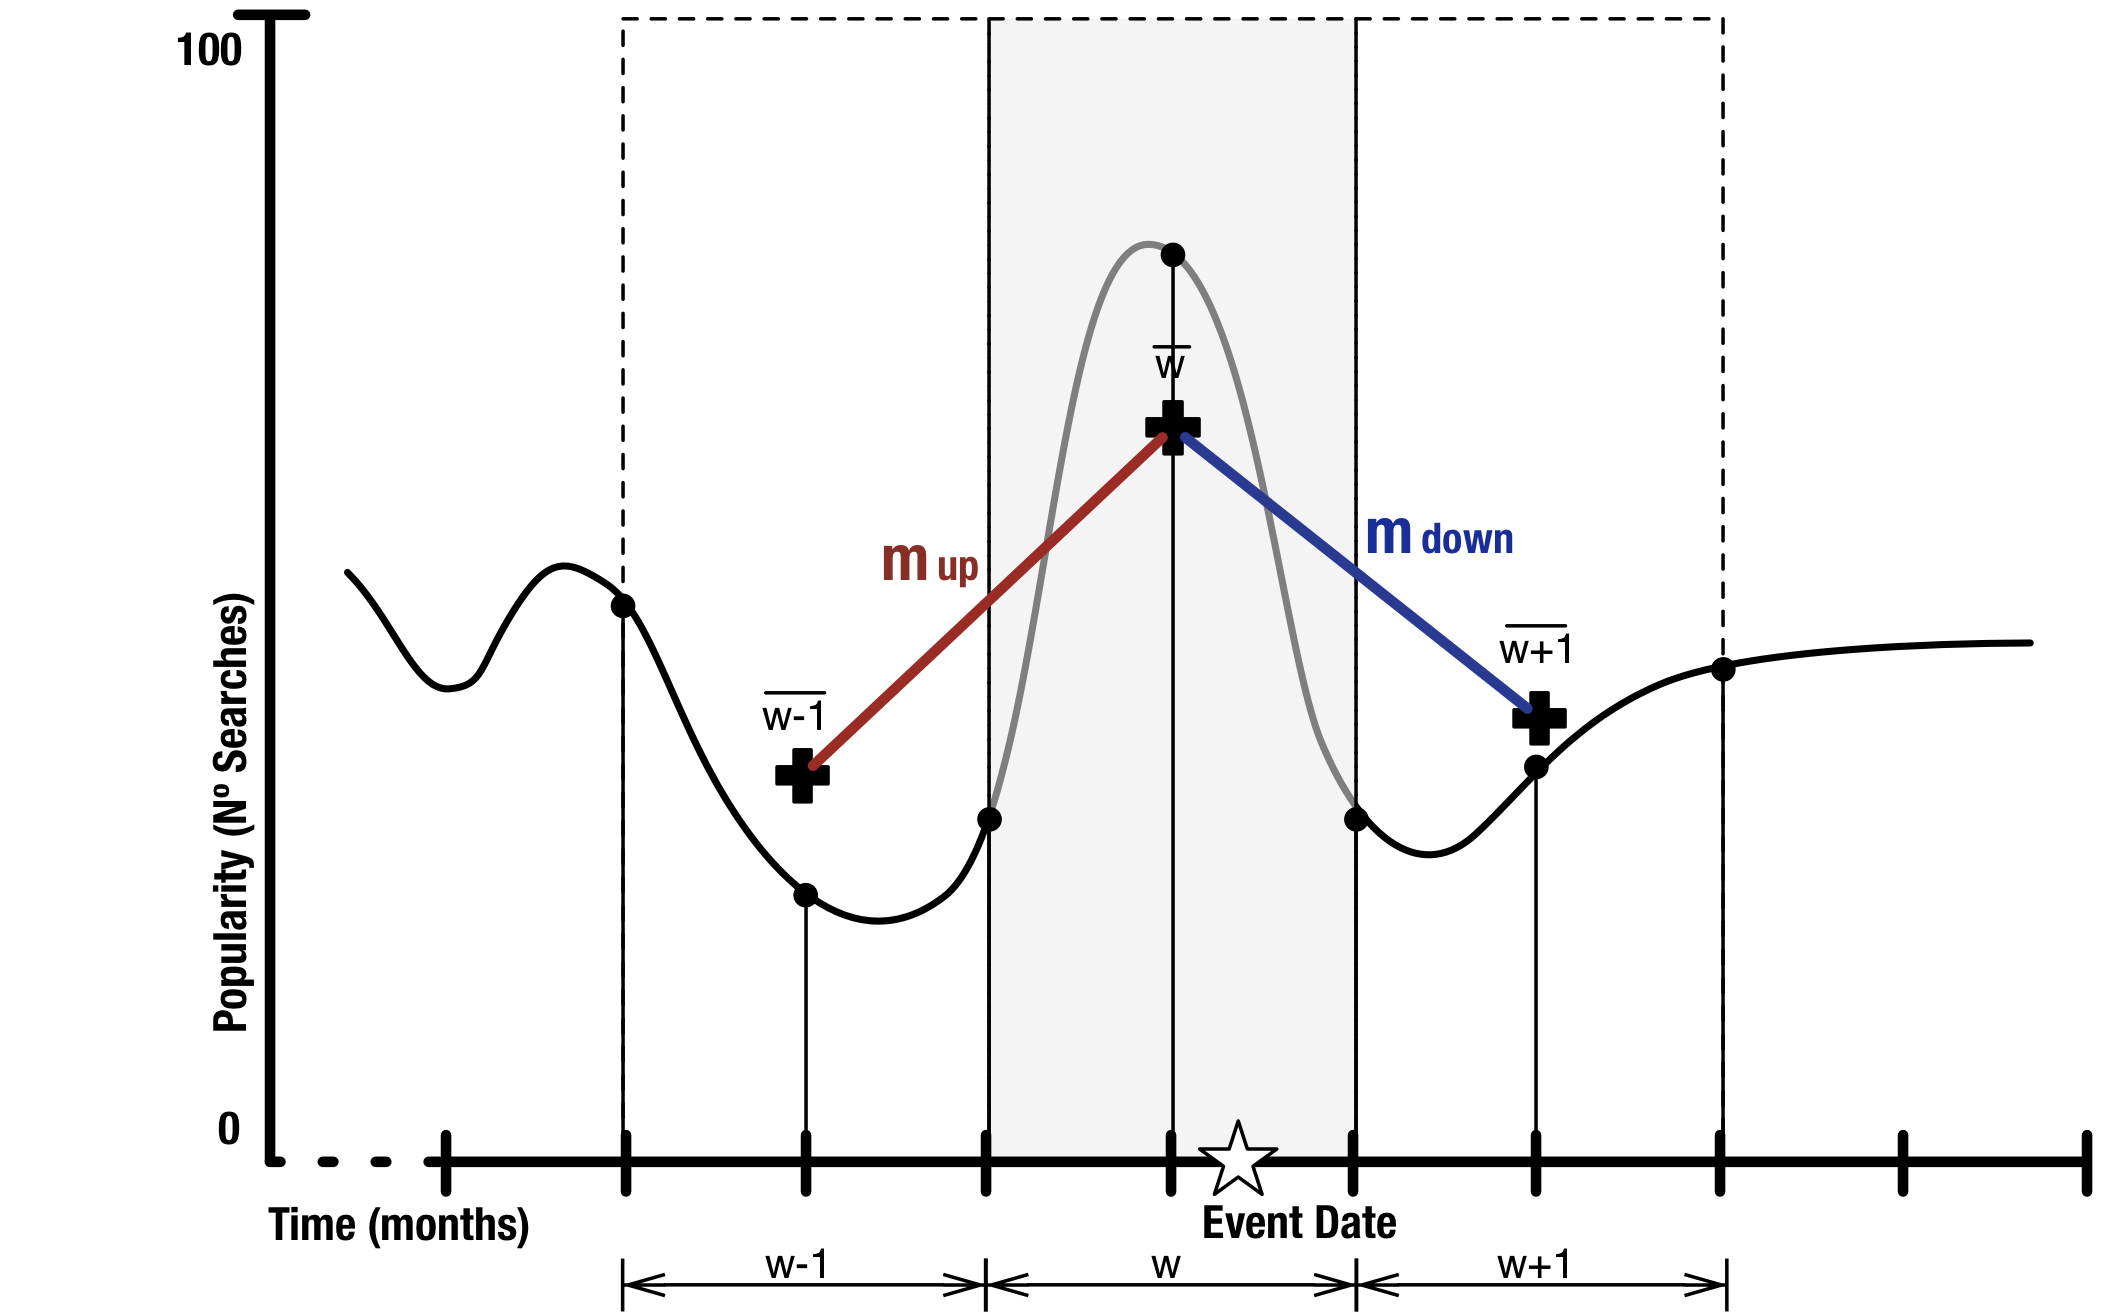
\includegraphics[width=0.7\textwidth]{figure/PopularityMeasure}
\caption{Popularity diagram of a considered event. On the x-axis is represented the time, and on the y-axis the magnitude of the popularity score. The star indicates when the event occurred. Given the discrete nature of the used platforms, the center of time window can be placed next to the day of the event.}
\label{fig:PopularityMeasure}%\end{figure}
\end{figure}

The procedure for getting $P_{peak}(e_i)$ is depicted in Fig.~\ref{fig:PopularityMeasure}. Using the label of an entity $e_i$, we obtain a list of pairs $[t, P]$ where $P\in[0,100]$ is the popularity score of an entity at the instant of time $t$. Afterward we create three consecutive and equally long temporal windows around $t$, the first one $w_{t}$ containing the date itself, another one just immediately behind $w_{t-1}$ and a last one after the previous two $w_{t+1}$. 
In a next step we approximate the area inside the regions by calculating the average of the points contained in them, obtaining $\overline{w-1}$, $\overline{w}$ and $\overline{w+1}$. The slopes of the lines between $\overline{w-1}$ and $\overline{w}$, and $\overline{w}$ and $\overline{w+1}$ give the values $m_{up}$ and $m_{down}$ respectively, which are normalized and combined into a single score for measuring how significant the variation in volume of searches was for that studied entity label. When aggregating those two gradients, we scored $m_{up}$ higher in order to emphasize the irruption of a change, more than the posterior distribution of the search term.
%\todo{GR:better phrase this part. This is a pure approximation btw}

By empirically studying the distribution of the popularity scores of the entities belonging to a newscast, we have observed that it follows a Gaussian curve. This fact will help us to better filter out popularity scores that do not trigger valid conclusions and therefore improving the merging of the ranking produced by the previous functions with the outcome from the popularity peaks detection algorithm. 

\subsubsection{Expert Rules Function}
%\todo{GR: dunno if it's propoer having this here, before the entire explaination. Most of the section should be moved later in the settings - supervised thing}
The knowledge of experts in the domain, like journalists or newscast editors can be materialized in the form of rules that correct the scoring output produced by former ranking strategies. The antecedent of those rules is composed by entity entity features such as type, number of documents where the entities appear, or the Web source from where documents have been extracted, while the precedent involves the recalculation of the scoring function according to the following equation: $S_{expert}\left ( e \right ) =  S_{F-1}\left ( e \right ) *Op _{expert}$, being $Op _{expert}$ a factor which models the domain experts' opinions about the entities that match in the antecedent.


%%%%%%%%%%%%%%%%%%%%%%%%%
%%%  5. Gold Standard %%%
%%%%%%%%%%%%%%%%%%%%%%%%%
\section{Gold Standard for Evaluating Newscast Semantic Snapshot}
\label{sec:GoldStandard}
We are interested in evaluating ranking strategies for generating semantic snapshots of newscasts, where each snapshot is charactherized by a set of named entities. We narrowed down the selection of named entity types to Person, Organisation, and Location, since they can be directly translated in \textit{who}, \textit{what}, \textit{when}, a subset of the 5Ws well-known questions in the journalisms. To the best of our knowledge there is no evaluation dataset suited to this context. The title of the newscasts and the breakdown figures per entity type are shown in Table~\ref{table:entitydistribution}. The dataset is freely available\footnote{\url{https://github.com/jluisred/NewsConceptExpansion/wiki/Golden-Standard-Creation}}.

%\vspace{-1.5em}
\begin{table}
\begin{tabular}{| p{6cm} | l| l| l| l|}
  \hline
  \textbf{Newscast Title} & \textbf{Person} & \textbf{Organisation} &\textbf{Location} & \textbf{Total} \\
    \hline
  Fugitive Edward Snowden applies for asylum in Russia & 11 & 7 & 10 & 28 \\
    \hline
 Egypt's Morsi Vows to Stay in Power & 4 & 5 & 4 & 17 \\
    \hline
 Fukushima leak causes Japan concern & 7 & 5 & 5 & 13\\
    \hline
 Rallies in US after Zimmerman Verdict & 9 & 2 & 8 & 19 \\
    \hline
 Royal Baby Prince Named George & 15 & 1 & 6 & 22 \\
    \hline
    \textbf{Total}  & 46 & 20 & 33 & 99\\
  \hline
\end{tabular}
\caption[Table caption text]{Breakdown entity figures per type and per newscast.}
\label{table:entitydistribution}
\end{table}

%\vspace{-2em}
\subsection{Newscast Selection}
We randomly selected 5 newscasts from the BBC One Minute World News website\footnote{\url{http://www.bbc.com/news/video_and_audio/}}. Each newscast lasted from 1 to 3 minutes. The selection covered a wide range of subjects specifically: politics, armed conflicts, environmental events, legal disputes, and social news. 
%The intention behind this topic choice was to fit international audiences, since we planned to perform a user study with international participants. 
Subtitles of the videos were not available; therefore, a member of the team manually transcribed the speech in the newscasts.
%After obtaining the transcriptions, the following steps were performed in order to obtain a set of unbiased candidate entities. 

\subsection{Newscast Semantic Annotation}
The annotation process involved two annotators and one expert of the domain. The output of this stage is a list of entity candidates. The two annotators were asked to detect for each newscast entities from: 
\begin{description}
\item[subtitle]: the newcast subtitle;
\item[image]: every time a recognisable person, organisation or location was portrayed in the newscast, the entity was added to the list;
\item[image captions]: the named entities appearing in such tags, such as nametag overlays, were added to the candidate set;
\item[external documents]: the two annotators were allowed to use Google Custom Search to look for articles related to the video. The query followed the pattern: title of the newscast, date. The sources were considered: The Guardian, New York Times, and Al Jazeera online (English). The results were filtered of one week time, where the median is represented by the day when event took place.
\end{description}

A journalist, with more than 6 years of experience as a writer and editor for important American newspapers and websites, acted as the expert of the domain. He was asked to watch the newscasts and to identify for each the entities either mentioned or not that better serve the objective of showing interesting additional information a final reader. The expert did not have access to the candidate set built by the two annotators, and he was completely free to suggest any named entity he wanted. 

\subsection{Quality control and Ranking}
A quality control refined the set of entities coming from the previous stage, eliminating all named entity duplicates and standardising names. 
%For example, when we had ``Barack Obama'' as an entity and ``Obama'' as another entity we eliminated the shorter one and left the complete name. A total of 99 entities were obtained from all videos. 
We then conducted a crowdsourcing survey with the objective to gather information about the degree of interestingness of the entities for each newscast. Based on \cite{vonBrzeski:2007:LCU:1321440.1321537} we define interestingness whether an entity is interesting, useful or compelling enough to tear the user away from the main thread of the document. Fifty international subjects participated in this online study. They responded an online call distributed via email and social networks. Their age range was between 25 and 54 years with an average age of 30.3 (standard deviation 7.3 years). 18 participants were female and 32 were male. Most of the participants were highly educated and 48 of them had either a university bachelor degree or a postgraduate degree. The main requisite for participation was that they were interested in the news and followed the news regularly, preferably through means that include newscasts.
During the interview participants were asked to choose at least 3 out of 5 videos according to their preferences. Then they were shown each one of the newscasts. Then they were asked to rate whether they would be interested in receiving more information about the named entities in the context of the news video and on a second screen or similar application. All the named entities from the candidate set related to the last seen video were shown in a list with ratio buttons arranged in a similar way to a three-point Likert-scale. The possible answers were ``Yes'' ``Maybe'' and ``No''. 

%\todo{JL:Period of time where the events were happening?}

%%%%%%%%%%%%%%%%%%%%%%%%%%%%%%%%%%%%%%%%%%%%%%%%
%%%  6. Experimental Settings and Evaluation %%%
%%%%%%%%%%%%%%%%%%%%%%%%%%%%%%%%%%%%%%%%%%%%%%%%
\section{Experimental Settings and Evaluation}
\label{sec:Evaluation}

In this section we measure the effectiveness of our approach for building the NSS of a newscast against the gold standard shown before. We present the measures considered to carry out the study, we describe the experimental settings, and we conclude with the results.

\subsection{Measures}
Inspired by similar studies in Web search engines, we have based our evaluation procedure in measures which try to find as many relevant documents as possible, while keeping the premise that the top ranked documents are the most important. In order to summarize the effectiveness of a the different algorithm across the entire collection of queries considered in the gold standard, we have considered different averaging measures that are listed below:

\begin{itemize}
\item Mean precision/recall at rank N. It is probably the most used measure in information retrieval tasks. It is easy to understand and emphasize the top ranked documents. However it does not distinguish between differences in the rankings at positions 1 to p, which may be considered important for some tasks. For example, the two rankings in Figure~\ref{fig:precisionRecall} will be the same when measured using precision at 10.
\item Mean average precision at N. Also called $MAP$, it takes in consideration the order of the relevant items in the top N positions and is an appropriate measure for evaluating the task of finding as many relevant documents as possible, while still reflecting the intuition that the top ranked documents are the most important.
\item Average Normalized Discounted Cumulative Gain $MNDCG$ at $N$. The Normalized Discounted Cumulative Gain is a popular measure for evaluating Web search and related applications~\cite{croft2010}. It is based on the assumption that there are different levels of relevance for the documents obtained in results. According to this, the lower the ranked position of a relevant document the less useful it is for the user, since it is less likely to be examined. 
\end{itemize}

As the relevant documents in our gold standard are scored in relevance for the user, we have mainly focused on the last mesure since it can provide a more exhaustive judgement about the adequacy of the generated NSS. Concerning the evaluation point N, we have performed an empirical study over the whole set of queries and main ranking functions observing that from $N=0$ $MNDCG$ decreasingly improves until it reaches a stable behavior from $N=10$ on. Finally, we will not perform measures in terms of efficiency. Even this kind of studies are easier to quantify, this falls outside the scope of this paper.
\begin{figure}[h!]
\centering
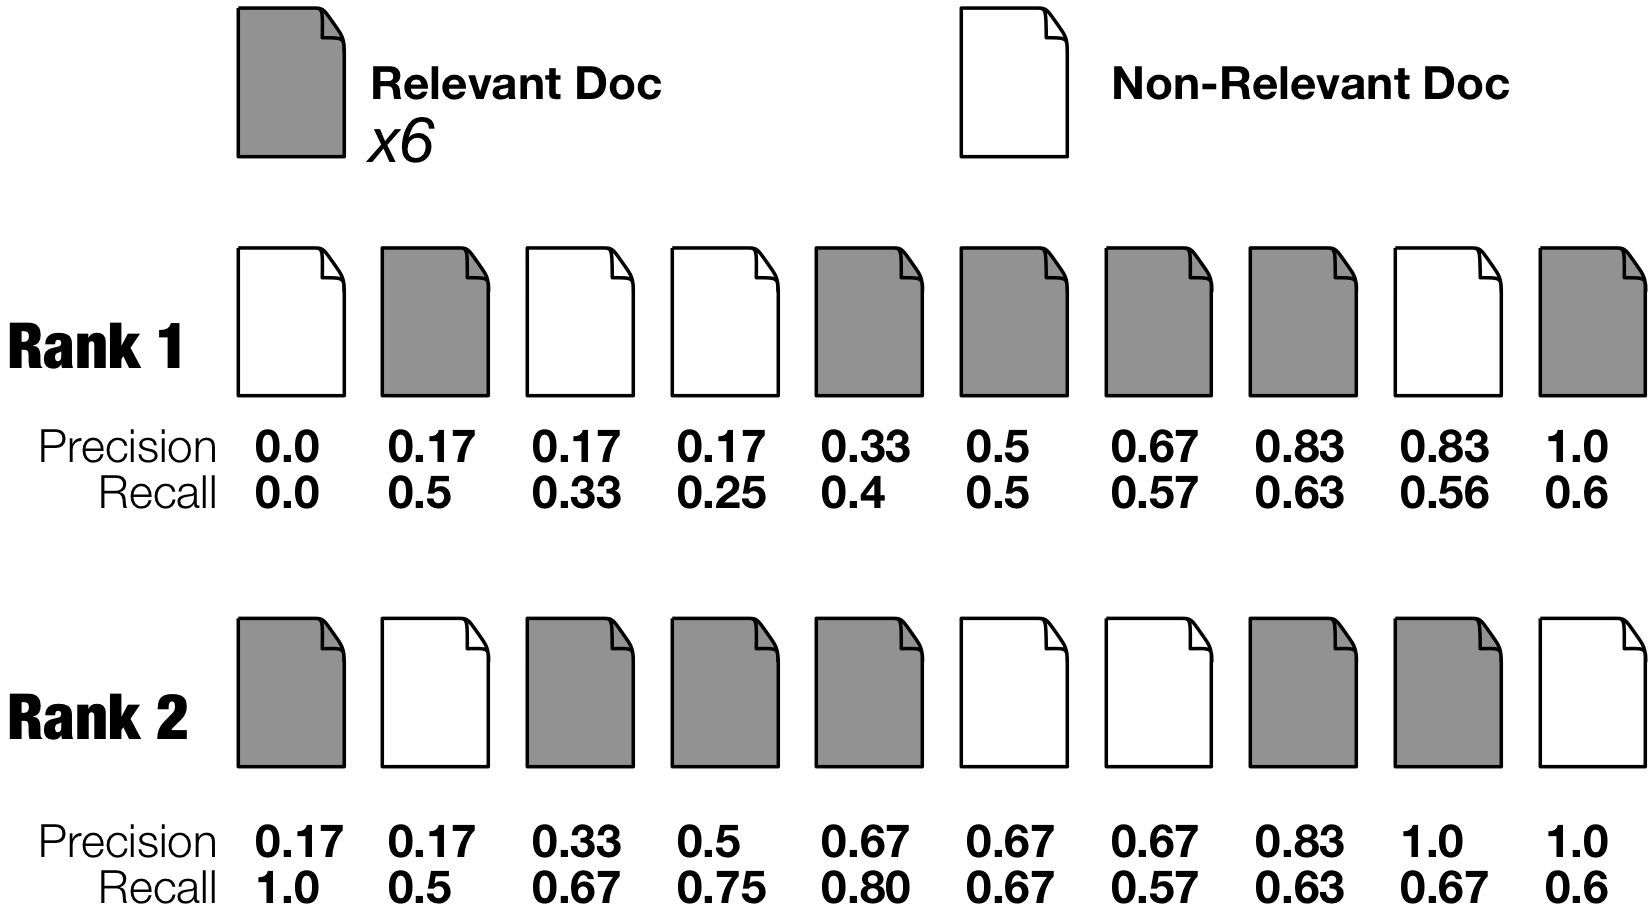
\includegraphics[width=0.8\textwidth]{figure/precisionRecall}
\caption{Inability of $P/R$ for considering the order of the relevant documents: rankings 1 and 2 share the same Precision and Recall at 10 .}
\label{fig:precisionRecall}%\end{figure}
\end{figure}

\subsection{Experimental Settings}
\label{sec:experimentalSettings}
\subsubsection{Document retrieval}
We have relied on the Google Custom Search Engine (CSE) API service\footnote{\fontsize{8pt}{1em}\selectfont  \url{https://www.google.com/cse/all}} by launching a query with the parameters specified by $q= \left [ \text{h}, \text{t} \right ]$. Apart of the query itself, the CSE engine considers other parameters that need to be tuned up. First, due to quota restrictions the maximum number of retrieved document is set to 50. But in addition, we have also considered 3 different dimensions that influence the effectiveness in retrieving related documents:
\begin{enumerate}
 \item Web sites to be crawled. Google allows to specify a list of web domains and subdomains where documents can be retrieved. This reduces the scope of the search task and, depending on the characteristics of the considered sources, influence the nature of the retrieved items: from big online newspapers to user generated content. At the same time, Google allows to prioritize searching over those whitelists while still considering the  whole indexed Web. Based on this, in our study we considered five possible values for this parameter:
 \begin{description}
  \item[Google]: search over the whole set of Web pages indexed by Google.
  \item[L1]: A set of 10 internationals English speaking newspapers.\footnote{\fontsize{8pt}{1em}\selectfont  \url{http://en.wikipedia.org/wiki/List_of_newspapers_in_the_world_by_circulation}}
  \item[L2]: A set of 3 international newspapers used in the gold standard creation.
  \item[L1+Google]: Prioritize content in Newspaper whitelist but still consider other sites.
  \item[L2+Google]: Prioritize content in Lilia's whitelist but still consider other sites.
 \end{description}
 \item Temporal dimension. This variable allows to filter those documents which are not temporarily close from the day where the newscast was published. Assuming that the news item is fresh enough, this date of publication will also be fairly close to the day the event  took place. Taking $t$ as a reference and increasing the window in a certain amount of days $d$, we end up having $Time_{Window}=\left [ \text{t}-d, \text{t}+d \right ]$ The reason why we expand the original event period is because documents concerning a news event are not always published during the time of the action is taking place but some hours or days after or before. The final $Time_{Window}$ could vary according to many factors such as the nature of the event itself (whether it is a brief appearance in a media, or part of a longer story with more repercussion) or the kind of documents the search engine is indexing (from very deep and elaborated documents that need time to be published, to short post quickly generated by users). In this study we have considered two possible values for it: 2 weeks and one week temporal windows.
 \item In addition, Google CSE makes possible to filter result according to the Schema.org types; for our experiments we use the following settings: [NoFilter, Person\&Organization]
\end{enumerate}

%That makes in total $5 * 2 * 2 = 20$ different parameter configurations that will be considered  that we will study in the Section~\ref{sec:evaluation} in order to discover which configuration optimizes the expansion algorithm.

\subsubsection{Semantic Annotation}
\label{sec:settingsFilteringClustering}
We use~\cite{RIZZO:2014} which applies machine learning classification of the entity type given a rich feature vector composed of a set of linguistic features, the output of a properly trained Conditional Random Fields classifier and the output of a set of off-the-shelf NER extractors supported by the NERD Framework.\footnote{\url{http://nerd.eurecom.fr}} We used it as an off-the-shelf entity extractor, using the offered classification model trained over the newswire content.

\subsubsection{Annotation Filtering and Clustering}
\label{sec:settingsFilteringClustering}
After some first trials it became evident that there were many non-pure named entities detected in the semantic annotation phase which are not well considered by viewers and experts. We have then applied three different filtering approaches:

\begin{description}
\item[F1]: Filter annotations according to their NERD type\footnote{\url{http://nerd.eurecom.fr/ontology}}. In our case, we keep only Person, Location, and Organization.
\item[F2]: It consists in getting ride of entities with confidence score under first quarter of the distribution.
\item[F3]: Intuitively, people seem to be more attracted by proper names than general terms. Those names are normally capitalized. This filter keeps only named entities matching this rule.
\end{description}

By concatenating those filters, we obtain the following combinations: F1,  F2,  F3,  F1\_F2,  F1\_F3, F2\_F3, F1\_F2\_F3 ). In order to reduce the number of runs, we did a first preselection of filters by setting the rest of steps of the approach to default values and averaging the scores obtained over the different queries. We ended up discovering that 3 of the filters (F1 and F3, and the combination F1\_F3) were producing best results in the final MNDCG, 

\subsubsection{Semantic Annotation Ranking}
\label{sec:settingsAnnotationRanking}
For the current experiment we run both Frequency and Gaussian based functions, together with the orthogonal strategies based on popularity and expert rules. This makes a total of $2*2$ possible ranking configurations that will be considered and reported in result section. Regarding the particular details of the orthogonal functions, we have proceeded as follow:

\begin{description}
\item [Popularity] We have relied on Google Trends,\footnote{\url{https://www.google.com/trends}} which estimates how many times a search-term has been used in a given time-window. Since Google Trends gives results with a monthly temporal granularity, we have fixed the duration of such $w$ to 2 months in order to increase the representativity of the samples without compromising too much the validity of the selected values according with the time the event took place. With the aim of being selective enough and keep only those findings backed by strong evidence, we have filtered the entities with peak popularity value higher than $\mu+2*\sigma$ which approximately corresponds to a 2.5\% of the distribution. Those entities will have their former scores combined with the popularity values via the following equation: $S_{P}\left ( e \right ) =  R_{score}\left ( e \right ) +Pop_{peak}(e)^{2} $.
\item[Expert Rules] \textit{i)} Entity type based rules: we have considered three rules to be applied over the three entity types considered in the gold standard. The different indexes per type have been deduced by relying on the average score per entity type computed in the survey $\overline{Sgt}_{entityType}$. 
%with the average score all over the entities $\overline{S}_{GT}$, so $Op _{expert}=1+(\overline{Sgt}_{GT_{entityType}} - \overline{S}_{GT})$ . 
Organizations have gotten a higher weight ($Op _{expert}=0.95$), followed by Persons ($Op _{expert}=0.74$), and by Locations ($Op _{expert}=0.48$) that are badly considered and therefore lower ranked in general. \\
%-0.292803855
%- Organizations have the higher average score compared to the average, so they are eminently interesting for users. -0,05
%- Persons have a fair average compare to the mean, so they should be somehow promoted as well. -0,24
%- $GT_{Location}$ is quite low compared to the average so scores of entities from this type should be penalized. -0,52.
\textit{ii)} Entity's documents based rules: each entity has to appear at least in two different sources in order to become a candidate. All entities whose document frequency $f_{doc}(e_i)$ is lower than 2 are automatically discarded ($Op _{expert} = 0$).
\end{description}

\subsection{Results}
\label{sec:results}

Given the different settings for each phase of the approach ($N_{runs_{Collection}} * Runs_{Filtering} * Runs_{Ranking}$), we have a total of  $20 * 4 * 4 = 320$ different runs that have been launched and ranked according to $MNDCG_{10}$. In addition we have also executed two baseline approaches for comparing them with the better performing strategies in our approach. More details about them are shown below.

\subsubsection{Baseline 1: Former Entity Expansion Implementation}
As reported in the related work, a previous version of the News Entity Expansion algorithm was already published in~\cite{RedondoGarcia2014}. The settings are: Google as source of documents, temporal window of 2 Weeks, no Schema.org selected, no filter strategy applied, and only frequency based ranked function with no orthogonal appliances. Results are reported in Table~\ref{table:results} under the run id \textit{BS1}.
 
\subsubsection{Baseline 2: TFIDF-based Function}
To compare our absolute frequency and Gaussian based functions with other possible approaches already reported in the literature, we selected the well-known TF-IDF. It measures the importance an entity in a document over a corpus of documents $D$, penalizing those entities appearing more frequently. The function, in the context of the named entity annotation domain is as follows:
\begin{equation}
\begin{matrix}
tf(e_i,d_j) = 0.5 + \frac{0.5\times f_{a}(e_i,D)}{max\left \{ f_{a}(e_i',D) : e_i' \in d_j\right \}},   idf(e_i,d_j) = log\frac{\left | D \right |}{\left \{ d_j\in D  :  e_i\in d_j \right \}}
\end{matrix}
\end{equation}

%We consider to make some adjustment in the formal since in our case the ranking algorithm has to be able to expose the importance of an entity inside the whole corpus $D$, while by definition TF-IDF refers only to the importance of an entity inside a particular document. 

We computed the average of the TF-IDF for each entity across all analyzed documents, resulting in aggregating the different $tf(e_i,d_j) \times idf(e_i,d_j)$ into a single function $tfidf^{*}(e_i,D)$ via the function $S_{TFIDF}(e)= \frac{ \sum_{j=1}^{n}  tf(e,d_j) \times idf(e)} {|D|}$.  Results are reported in Table~\ref{table:results} under the run id \textit{BS2}.

\subsubsection{Launching the Experiments}

\begin{table}[h]
  \resizebox{12cm}{!} {

\begin{tabular}{llllllllllll}
\hline
\multicolumn{1}{|c|}{\multirow{2}{*}{Run}} & \multicolumn{3}{c|}{Collection} & \multicolumn{1}{c|}{\multirow{2}{*}{Filtering}} & \multicolumn{3}{c|}{Functions} & \multicolumn{4}{c|}{Result} \\ \cline{2-4} \cline{6-12} 
\multicolumn{1}{|c|}{} & \multicolumn{1}{c|}{Sources} & \multicolumn{1}{c|}{$T_{Window}$} & \multicolumn{1}{c|}{Schema.org} & \multicolumn{1}{c|}{} & \multicolumn{1}{c|}{Freq} & \multicolumn{1}{c|}{Pop} & \multicolumn{1}{c|}{Exp} & \multicolumn{1}{c|}{$MNDCG_{10}$} & \multicolumn{1}{c|}{$MAP_{10}$} & \multicolumn{1}{l|}{$MP_{10}$} & \multicolumn{1}{l|}{$MR_{10}$} \\ \hline
Ex0 & Google & 2W&   & F1+F3 & Freq &   & \checkmark & 0.666 & 0.71 & 0.7 & 0.37 \\
Ex1 & Google & 2W&   & F3 & Freq &   & \checkmark & 0.661 & 0.72 & 0.68 & 0.36 \\
Ex2 & Google & 2W&   & F3 & Freq & \checkmark & \checkmark & 0.658 & 0.64 & 0.6 & 0.32 \\
Ex3 & Google & 2W&   & F3 & Freq &   &   & 0.641 & 0.72 & 0.74 & 0.39 \\
Ex4 & L1+Google & 2W&   & F3 & Freq &   & \checkmark & 0.636 & 0.71 & 0.72 & 0.37 \\
Ex5 & L2+Google & 2W&   & F3 & Freq &   & \checkmark & 0.636 & 0.72 & 0.7 & 0.36 \\
Ex6 & Google & 2W&   & F1+F3 & Freq &   &   & 0.626 & 0.73 & 0.7 & 0.38 \\
Ex7 & L2+Google & 2W&   & F3 & Freq &   &   & 0.626 & 0.72 & 0.72 & 0.37 \\
Ex8 & Google & 2W&   & F1+F3 & Freq & \checkmark & \checkmark & 0.626 & 0.64 & 0.56 & 0.28 \\
Ex9 & L2+Google & 2W&   & F1+F3 & Freq &   & \checkmark & 0.624 & 0.71 & 0.7 & 0.37 \\
Ex10 & Google & 2W&   & F1 & Freq &   & \checkmark & 0.624 & 0.69 & 0.62 & 0.32 \\
Ex11 & L1+Google & 2W&   & F3 & Freq &   &   & 0.623 & 0.7 & 0.72 & 0.37 \\
Ex12 & L2+Google & 2W&   & F3 & Freq &   & \checkmark & 0.623 & 0.68 & 0.66 & 0.35 \\
Ex13 & L2+Google & 2W&   & F3 & Freq & \checkmark & \checkmark & 0.623 & 0.61 & 0.56 & 0.3 \\
Ex14 & L2+Google & 2W&   & F3 & Freq &   &   & 0.62 & 0.69 & 0.74 & 0.4 \\
Ex15 & L1+Google & 2W& \checkmark & F1+F3 & Freq &   & \checkmark & 0.617 & 0.69 & 0.66 & 0.34 \\
Ex16 & L2+Google & 2W&   & F1 & Freq &   & \checkmark & 0.616 & 0.68 & 0.62 & 0.32 \\
Ex17 & Google & 2W& \checkmark & F1+F3 & Freq &   & \checkmark & 0.615 & 0.7 & 0.64 & 0.32 \\
Ex18 & L1 & 2W& \checkmark & F3 & Freq & \checkmark & \checkmark & 0.614 & 0.65 & 0.6 & 0.32 \\
Ex19 & L1+Google & 2W&   & F1+F3 & Freq &   &   & 0.613 & 0.72 & 0.72 & 0.38 \\
Ex20 & L1+Google & 2W&   & F1+F3 & Freq &   & \checkmark & 0.613 & 0.7 & 0.66 & 0.35 \\
... & ...  & ... & ...  & ...  & ...  & ... & ...  & ...  & ...  & ...  & ...  \\
Ex78 & Google & 2W& \checkmark & F1+F3 & Gaussian &   & \checkmark & 0.552 & 0.66 & 0.66 & 0.34 \\
Ex80 & L2+Google & 2W& \checkmark & F1+F3 & Gaussian &   & \checkmark & 0.55 & 0.69 & 0.7 & 0.36 \\
Ex82 & L1 & 2W& \checkmark & F3 & Gaussian &   & \checkmark & 0.549 & 0.68 & 0.64 & 0.33 \\
... & ...  & ... & ...  & ...  & ...  & ... & ...  & ...  & ...  & ...  & ...  \\
BS2 & Google & 2W&   &   & Freq &   &   & 0.473 & 0.53 & 0.42 & 0.22 \\
... & ...  & ... & ...  & ...  & ...  & ... & ...  & ...  & ...  & ...  & ...  \\
BS1 & Google & 2W&   &   & TFIDF &   &   & 0.063 & 0.08 & 0.06 & 0.03 \\
\end{tabular}
}
\caption[Table caption text]{Executed runs and their configuration settings, ranked by $MNDCG_{10}$}
\label{table:results}
\end{table}

In Table~\ref{table:results} we present the top 20 runs for our approach in generating NSS, together with some lower configurations at position 78 and following that are worth to be reported and the scores of the baseline strategies. We summarize the main findings of the experimental settings and evaluation as follows:
\begin{itemize}
\item Our best approach has obtained a $MNDCG_{10}$ score of 0.662 and a $MAP_{10}$ of 0.71, which are reasonably good in the document retrieval domain.
\item Our approach performs much better than BS1 and by far better than BS2. The very low score of this last baseline is explained in the fact that tradicional TF-IDF function is designed to measure the relevance of an item referred to the document that contains it and not to the whole collection. In addition, the absence of filters drop drastically the scores.
\item Regarding the Document Retrieval step, we see that using Google as source alone of together with other WhiteList gives better results than restricting only to particular whitelist. The biggest $T_{Window}$ of 2 weeks performs better in all cases, while the use of Schema.org does not bring anything back except when is applied over the Gaussian function (see runs 78, 80, 82) where it turns to be an influent factor.
\item the best Filter strategy is F3, followed by the combination F1\_F3. In conclusion, capitalization is a very powerful tool for making a first candidate list with those entities that a priori users consider more interesting.
\item The absolute frequency function performs better than the Gaussian in all top cases.
\item The Expert Rules based function improves the final NSS for almost every configuration possible.
\item Popularity based function does not seem to improve significantly the results. However, a further manual study of the promoted entities has revealed that in fact, the method is bringing up relevant entities like for example \textit{David Ellsberg}\footnote{\url{http://en.wikipedia.org/wiki/Daniel_Ellsberg}} for the query ``Fugitive Edward Snowden applies for asylum in Russia''. This entity is barely mentioned in some of the collected documents, but \textit{David Ellsberg}'s role in the newscast is quite representative since he published an editorial with high media impact in The Guardian praising the actions of Snowden in revealing top-secret surveillance programs of the NSA. 
\end{itemize}

%%%%%%%%%%%%%%%%%%%%%%%
%%%  5. Conclusion  %%%
%%%%%%%%%%%%%%%%%%%%%%%

\section{Conclusion}
\label{sec:Conclusion}
In this paper we have presented an approach for automatically generating Newscast Semantic Snapshot. The followed approach is able to enlarge the niche of initial newscast content, retrieving and analyzing event-related documents from the Web. The bag of retrieved documents, together with the newscast transcript, is processed with the objective of extracting named entities referring to name of people, organizations, and locations. By increasing the size of the document set to analyze, we increase the completeness of the context and the representativeness of the list of entities, reinforcing relevant entities and finding new ones that are potentially interesting inside the context of that news item. The named entities are then ranked according to the entity appearence in the sampled collection of documents, popularity of the entity on the Web, and experts' rules. We benchmarked the entire workflow against a gold standard, which is also proposed in this paper. The evaluation has showed the strenght of this approach, holding an $MNDCG_{10}$ score of 0.666 against.
%that we can successfully expand the initial set of recognized entities with more relevant concepts not detected by pure named entity recognition approaches and produce a more accurate ranking of important concepts that brings forward entities which user are more interested about.

Future research interests include tailoring the entity ranking functions to particular news categories: sport, politics, regional, international, opinion. We are investigating the role of entity relations in generating of the Newscast Semantic Snapshot: usually entities are linked by tight relations extracted from a knowledge base, or simply from the documents collected, in order to generate a directed graph of entities instead of a list. We also plan to refine the ranking process, applying supervised techniques (Learning to Rank) that tailor the solution on particular domains. 
%We expect that applying it the performance of the approach will improve, depending on the domain explored in the gold standard. 
In the investigation we have conducted, we have encountered a few missing entities in the gold standard that were not identified because of human limitations when exhaustivelly covering the whole semantic picture of the newscast. We then plan to use our approach as a means to suggest relevant entities in the process of the gold standard creation.

%%%%%%%%%%%%%%%%%%%%%%%%%
%%%  Acknowledgments  %%%
%%%%%%%%%%%%%%%%%%%%%%%%%

\section*{Acknowledgments}
This work was partially supported by the European Union's 7th Framework Programme via the project LinkedTV (GA 287911).

%%%%%%%%%%%%%%%%%%%%%%
%%%  Bibliography  %%%
%%%%%%%%%%%%%%%%%%%%%%
\bibliographystyle{abbrv}
\bibliography{NewsConceptExpansion}

\end{document}
